%!TEX root = ../Main.tex

\section{Data}\label{sec:chapter3}

By effectively isolating the systematic risk associated with the volatility-of-volatility, it can be shown that the difference between the current returns variation (approximated by $RV$) and the markets risk-neutral expectation of future returns variation (approximated by IV) is a useful predictor of the future returns \textit{[BTZ 2009]}. Moreover, as shown above, we can construct the additional predictor SRP as a byproduct of these measures. We thus need reliable raw data to build the $RV^{U/D}$ and $IV^{U/D}$. The data used in this study is available through the Wharton Database. Specifically, we use the 3-month Treasury Bill rate ad our risk-free rate, the S\&P 500 composite index as a proxy for the aggregate market portfolio, 5-minute intraday S\&P 500 data and option data.

\subsection{Excess Returns}
In order to document the prediction power of $VRP^{U/D}$ and $SRP$ for monthly excess equity market returns, we use the S\&P 500 composite index as a proxy for the aggregate market portfolio. Next, we construct the excess returns by subtracting 3-month T-Bill rates from the annualised log-returns of the S\&P 500 composite index. 
\begin{equation}
r^e_t=ln(1+R_t) \times 12 - ln(1+R_t^f)
\end{equation}
where $R_t= \frac{S_t-S_{t-1}}{S_{t-1}}$ is the equity return and $R_t^f$ is the risk-free rate. 

\vspace{4mm}
Both the S\&P 500 composite index and the 3-month T-Bill rate series have been gathered from the CRSP database and we focus our analysis on the 2007-2017 sample period. 

\subsection{RV: High Frequency Data}
To build the daily $RV^{U/D}$s series, we use 5-minute intraday S\&P 500 data and, once again, we focus on the 2007-2017 sample period. The data is available through the Wharton Database.

\vspace{4mm}
For what concerns the 2007-2008 period, we have gathered tick data from the TAQ database, and subsequently proceeded to delete any duplicate and zero entries to obtain more consistent data. Finally, to obtain 5-minute data and overcome the issue of irregularly spaced data points we have created 5-minute bins by using the median. We have preferred to create these 5-minutes bins with the median rather than the mean value, as the former is more robust to outliers.  
For what concerns the 2008-2017 period we have obtained minute-data from the Wharton database. For both datasets, we averaged the market's bid and ask quotes in order to obtain an average S\&P 500 level. Finally, we have merged these two datasets to create an unique 5-minute intraday dataset comprising the whole period. We have dealt with missing values by recurring to interpolation.

\vspace{4mm}
We obtain the total realized variances by adding up the sum of the 5-minute squared log-returns and the daily squared overnight returns. We then decompose the total realized variances into their upside and dowside components with respect to the threshold $\kappa$. By construction we have that total realized variance is obtained by adding the downside ($RV^D$) and the upside realized variance ($RV^U$). 
The three series are scaled such that the average total realized variance series matches the unconditional variance of the S\&P 500 returns.


\subsection{IV: Options Data}
All of the data used for this computation is taken by OptionMetrics. From 'Option Prices' we downloaded the SPX European call and put options from 2007 to 2017 included. For the same period, we got zero curves from 'Zero Coupon Yield Curve' and, finally, from 'Index Dividend Yield' we downloaded the continuously compounded S\&P500 dividend yield.

\vspace{4mm}
Since not all the options give us reliable information about the market, we decided to apply some preliminary standard filtering procedures to delete illiquid options. In particular:
\begin{itemize}
    \item we computed the mid price as the average between bid price and ask price. Then we deleted the options with mid price below $3/8\$$;
    \item we deleted all the options with too long ($>$1 year) or too short ($<$7 days) time-to-maturity;
    \item we deleted all the options that have not been traded for more than three days in a row.
\end{itemize}

Since the tenors of the zero curves do not match the maturities of the options, we interpolated linearly the continuously compounded zero-coupon rates to solve this issue.


\subsection{Summary Statistics}

In the following we compare our data to \textit{Fenou's [2015]} data through the use of the summary statistics presented by the original paper. Before going into detail we would like to mention that our analysis presents several limitations with respect to the dataset, reflected in the summary statistics. Firstly we did not have the same time period of data available, limiting our analysis to the years 2007 to 2017 compared to 1996 to 2015. Secondly, the daily variables are aggregated to periods between one month and one year for the models and unfortunately we were uncertain which aggregation period was presented in the reported summary statistics.  Thirdly, we assumed the aggregation periods were constructed overlapping but can not be certain of this. Hence were not able to replicate the exact summary statistics that the authors presented and can not assume that our replication dataset matches that of the original paper. As a consequence, we limit ourselves to comparing the variables in their relative size to one another.\\

The total variance risk premium and downside variance risk premium are on average positive over our sample period. The upside variance risk premium however is on average negative. This aligns both with the authors theoretical and empirical findings, assuming that investors dislike bad uncertainty and are hence willing to pay a premium to be hedged against variation in bad uncertainty and vice versa. The realized variance is on average positive over the sample period both for the upside and downside measure, as is the implied volatility. Excess returns were on average 0.46$\%$ per day.

Table \ref{table1} presents the summary statistics of the data used in our models. 

\begin{table}[h]
\begin{center}
\caption{summary statistics}
\label{table1}
\hspace*{-1cm}
\begin{tabular}{l|rrr|rr|rr|r}
\toprule
{} &  $VRP$ &  $VRP^{U}$  &   $VRP^{D}$  &   $RV^{U}$ &    $RV^{D}$ &    $IV^{U}$  &          $IV^{D}$ & excess return\\
\midrule
mean  &     0.067227 &    -0.034161 &     0.101388 &     0.147523 &     0.168599 &     0.112790 &     0.268409 &     0.460595 \\
std   &     0.250356 &     0.135721 &     0.165122 &     0.246959 &     0.321733 &     0.155481 &     0.347752 &     4.809556 \\
min   &    -3.344685 &    -1.812280 &    -1.532405 &     0.008506 &     0.004881 &     0.006662 &     0.043216 &   -35.874178 \\
max   &     1.911116 &     0.397544 &     1.513572 &     2.346593 &     3.166236 &     1.732368 &     3.522595 &    20.273505 \\
\bottomrule
\end{tabular}\hspace*{-1cm}\\
\end{center}
\textit{Notes:} This table reports the summary statistic for the variables used in our model. For representative purposes only the aggregation period of one months is displayed. The variables reported are in percentage and non-annualized.
\end{table}


The graph below shows the time series plot of the variance risk premia and its up and downside decomposition. 

\begin{figure}[h]
\centering
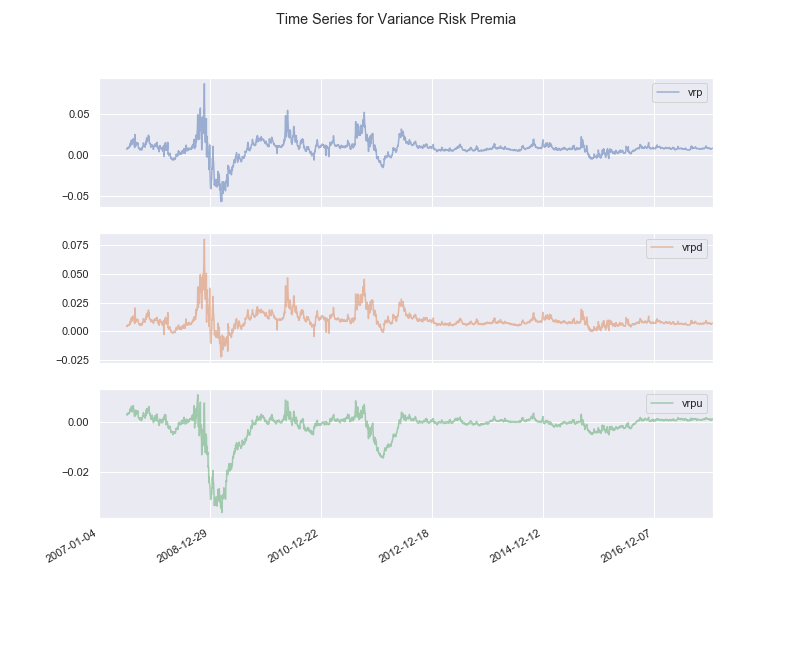
\includegraphics[scale = 0.4]{figures/TsPlots.png}
\caption{Time series plot of $VRP$, $VRP^U$ and $VRP^D$.}
\label{fig:TsPlot}
\end{figure}